\section{Approach}
\label{sec:approach}
Opinion summarization aims at generating abstractive 
summaries covering salient opinions expressed in multi-reviews.
Since the existing review corpus  $\mathbb{R}=(R^1, ..., R^E)$ about $E$ entities (e.g. products or restaurants) has no
reference summaries for training, we designed a weak supervised approach by constructing a semi-structured training dataset and summarizing with aspect-guided summarization models.
%Since there is no human-annotated data for training, our approach is weak supervised.


\subsection{Semi-structured Training Data Creation}
\label{sec:data}
%\JQ{exchange these two paragraphs?}
To avoid that some information in summary are missing in textual inputs or structured inputs,
% (as shown in \figref{fig:brief}),
we create a synthetic training dataset $\mathbb{D}$ 
by first sampling textual summary outputs and then sampling semi-structured inputs, including noisy OAs and noisy ISs corresponding to each output. The  intuition behind noising operations is to simulate the summarization process for real multi-reviews.
%sampling semi-structured inputs, including opinion-aspect pairs (OAs) and implicit sentences (ISs), and textual summary outputs. 
%IS is the sentence that we cannot extract OAs from, which can be regarded as the supplymentary of OAs.

Our method consists of four parts: 
%(1) we extract OAs and ISs from $R_e$%the reviews of entity $e$,
%(2) we sample a review as a summary $y$, 
%(3) {\em opinion-aspect pairs noising} selects proper OAs from $P^e$ to get noisy OAs for $y$,
%and (4) {\em implicit sentences noising} selects noisy sentences from $S^e$ 
%that different from ISs in $y$.
(1) \textbf{extracting OAs and ISs} from the other reviews $\overline{R^e}$ of $e$ to get the OAs group $\overline{P^e}$
and ISs group $\overline{S^e}$,
(2) \textbf{sampling a review} as a summary $y$ from all reviews $R^e$ of an entity $e$, 
(3) {\bf opinion-aspect pairs noising} which samples proper OAs from $\overline{P^e}$ to get {noisy OAs for $y$,
and (4) {\bf implicit sentences noising} which samples noisy ISs from $\overline{S^e}$. 
%The OAs an ISs in real multi-review can be seen as the noisy version of them in reference summary, 
%Taking noisy OAs and ISs as input simulates the process of summarization for OAs and ISs of multi-reivew.
% during generation. 
%The process is shown in \figref{fig:dm}.

We use $R^e=(r_1,...,r_M)$ to denote all reviews of an entity $e$. 
For a review $r$, we extract opinion-aspect pairs, 
$p=(p_{1},...,p_{d})$, 
expressing opinions of the reviewer towards aspects of the entity.
$p_i$ denotes the set of OAs for the $i$-th aspect.
$p_{i}=\{(o_{1,i}, f_1), ..., (o_{n,i}, f_n)\}$ where %$o_{j,i}=(o_j, a_i)$. 
$o_{j,i}$ is $j$-th OA pair of aspect $a_i$ 
and $f_j$ is the number of occurrences of $o_{j,i}$.
We use $s=(s_1,..., s_k)$ to denote the  ISs in review $r$. ISs usually express the specific information of the entity.
Thus, the review $r$ is represented by a set of OAs and a set of ISs.
The OAs of $R_e$ compose an OA group $P^e=(P_{1},...,P_{D})$, 
where $P_{i}=\{(o_{1,i},f_1), ..., (o_{N, i},f_N)\}$.
The ISs of $R_e$ compose an IS group $S^e=(s_1,..., s_K)$. 




\begin{figure}[th]
	\centering
	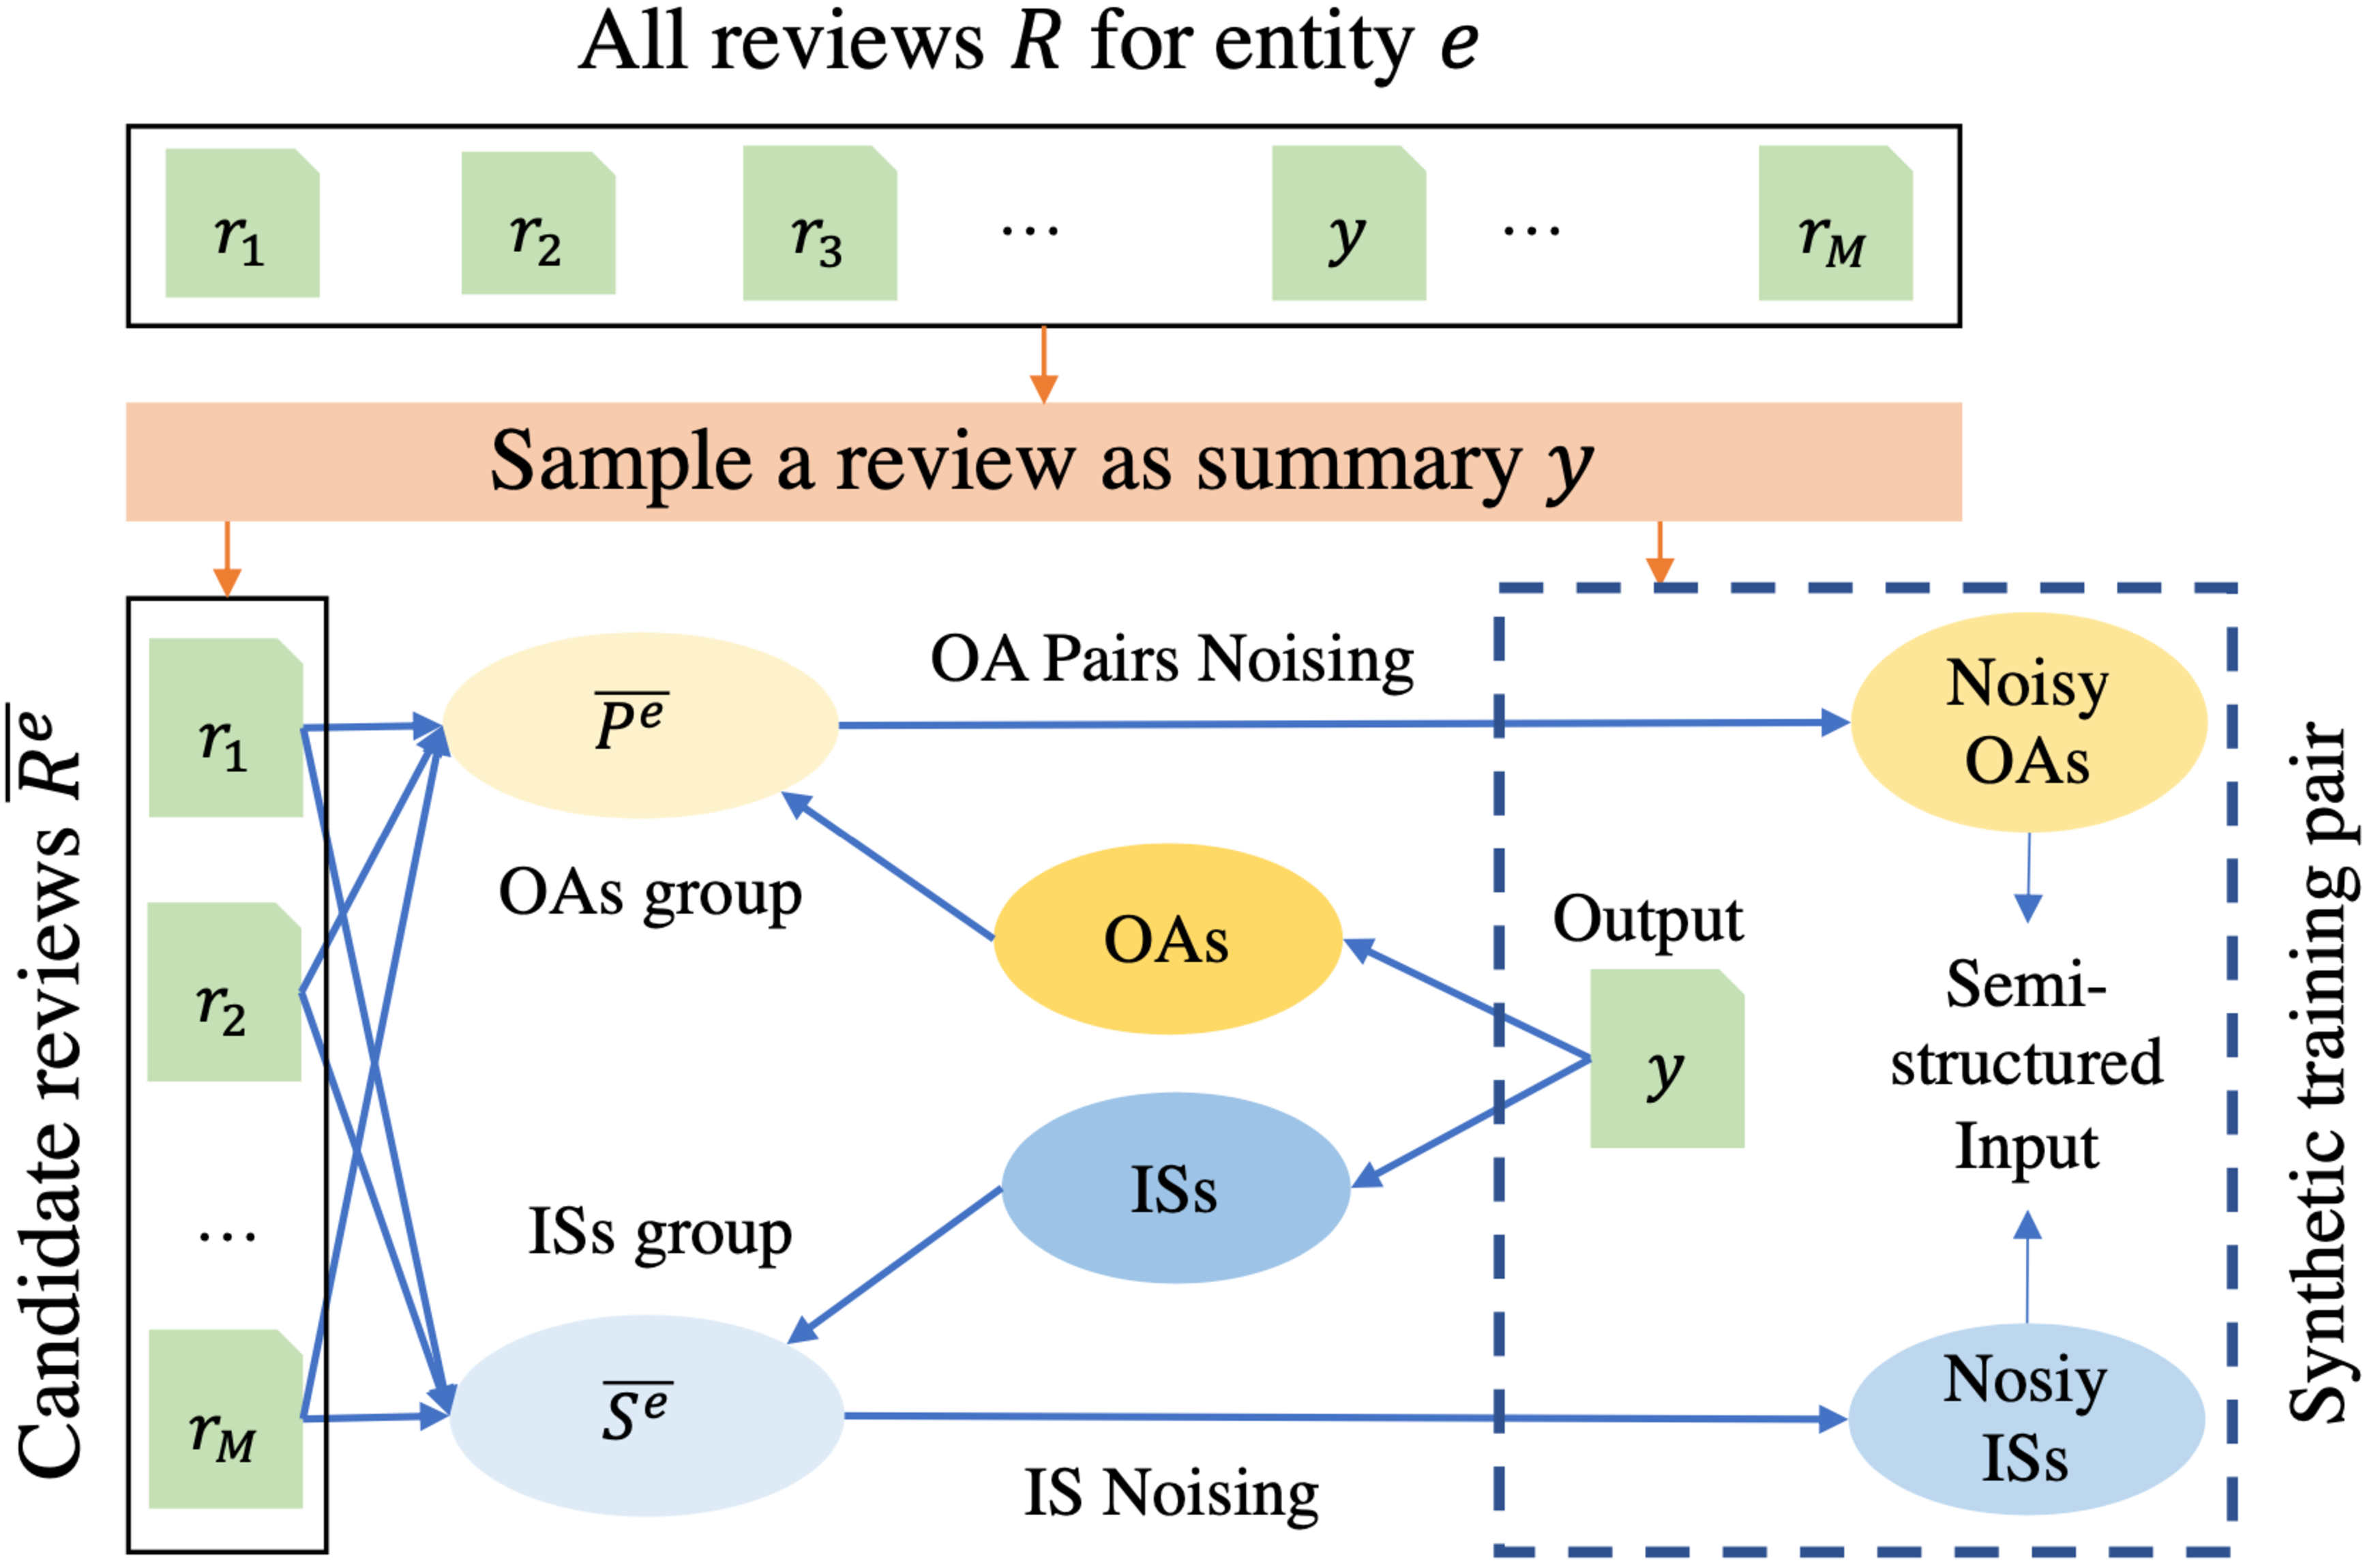
\includegraphics[width=0.9\linewidth]{./dm.pdf}
	\caption{Semi-structured training data creation.}
	\label{fig:dm}
\end{figure}

\textbf{Opinion-aspect Pairs Extraction.} 
%Aspect-based Sentiment Analysis (ABSA) task 
%~\cite{OpiMinHuL04,OpiMinDaiS19}
%can help extract opinion-aspect pairs.
%\KZ{I think no point talking about the above one since
%we didn't use it. Instead, talk about it in the related work.}
For every review, we utilize a rule-based MIN-MINER ~\cite{basicOpiMin20} to get the dependency parse trees of sentences first and then use a set of syntactic rules~\cite{aspect12} to extract OAs.
\cut{%%%%
We obtain OAs for every review in corpus by a rule-based
MIN-MINER~\cite{basicOpiMin20} . 
It gets the dependency
parse trees of sentences first and then uses a set of syntactic rules~\cite{aspect12} to extract opinion-aspect pairs.
~\footnote{It is flexible to use different opinion-aspect extractions.}
}%%%%

\textbf{Summary Sampling.} 
 %Wefollow~\citet{Denoise20} with sampling 
We take a sampled review of entity $e$ as {\em summary} ($y$) and the other reviews of $e$ as {\em candidate reviews} ($\overline{R^e}$).
%Similarly, 
During sampling, we ignore the reviews containing first-person singular pronouns
and non-alphanumeric symbols aside from punctuation~\cite{Denoise20}.
Besides, 
we ensure that 
all aspects of the summary 
can be found in $\overline{R^e}$.
This is more close to the fact that aspects in the summary are mostly
from its multi-review.
%We follow \citet{Denoise20} with sampling a review from the corpus as summary.
%The summary must be no first-person singular pronouns, 
%and no non-alphanumeric symbols aside from punctuation.
%We sample a review of entity $e$ as {\em summary},
$\overline{P^e}=(\overline{P}_{1},...,\overline{P}_{D})$ is the OAs of $\overline{R^e}$.
$\overline{P}_{i}=\{(o_{1,i},f'_1), ..., (o_{N, i},f'_{N})\}$ contains
the OA pair $o_{j,i}$ and the number of its occurrences $f'_j$.
 %\JQ{the last two sentences are not clear}

\textbf{Opinion-Aspect Pairs Noising.}
%\JQ{Add the intuition behind two directions}
There are two directions of opinion-aspect pairs noising: 
{\em exactly matched} (EM) OAs and {\em mismatched} (MM) OAs.
The noisy OAs from EM simulate the real summarization that
some aspects of summary are mentioned in different reviews.
The noisy OAs from MM reflect that the aspects of summary is the subset 
of the aspects of multi-review. We estimate the distributions of 
both kinds of OAs and the sampling size of them as follows.


For EM,
%give the OAs with aspect $a$ in summary $y$, 
%we extract exactly matched OAs from $\overline{P^e}$ of $y$, 
%of which the aspects are same as summary.
we extract OAs contraining the same aspects as summary from $\overline{P^e}$ as exactly matched OAs.
%The OAs in $\overline{P^e}$ with $a$ 
%different from summary are mismatched OAs.
Other OAs in $\overline{P^e}$ are mismatched OAs.
%Given a summary $y$ about entity $e$ as output,  we construct noisy OAs 
%for OAs in $y$ as input 
%by extracting some OAs of $e$ in terms of
{%\em exactly matched} (EM) aspects
%and {\em mismatched} (MM) aspects.
We get word representations from GloVe~\cite{glove}
%{https://github.com/stanfordnlp/GloVe}
%We take the average of the word embeddings in opinion (aspect)
%as opinion (aspect) embedding.
%The opinion-aspect pair embedding is the matrix consisting of opinion embedding
%and aspect embedding.
and take the average of word embeddings in an opinion-aspect pair
as {\em OA embedding}.
%The pairs in exactly matched OAs should be different from summary.
%The exactly matched OAs and mismatched OAs are sampled
%according to the distribution of cosine similarity (CS) 
%between OAs in multi-review and summary in development set,
%which resemble actual summarization of multiple reviews.
%\footnote{The development set in this work is created by human.}
%The noisy OAs from EM aspects simulate the real summarization that
%some aspects of summary are mentioned in different reviews.
As opinions on the same aspect of multiple reviews are mostly similar,
exactly matched OAs are sampled according to
the distribution of cosine similarity (CS) 
between exactly matched OAs of $\overline{P^e}$ and summary.
%The aspect $a$ in summary is represented as $\boldsymbol{p}_a$, 
$\boldsymbol{p}_i$ represents a set of OAs with aspect $a_i$ in summary,
which is the average of OA embedings of $a_i$.
 We compute the $CS$ scores between exactly matched OAs on $a_i$ and $\boldsymbol{p}_i$ as: $cs_j(a_i)=cosine\_sim(\boldsymbol{o}_{j,i}, \boldsymbol{p}_{i})$
where $\boldsymbol{o}_{j,i}$ is the embedding of $j$-th opinion-aspect pair of $a_i$ in exactly matched OAs.
We normalize the $CS$ scores of $a_i$
by $\widetilde{CS}=softmax(\mathbf{cs}(a_i))$. 
The $\widetilde{CS}$ denotes the probability distribution 
of OAs in an exactly matched aspect.
To create training data,
we sample OA pair from exactly matched OAs for an aspect
according to the distribution $\widetilde{CS}$. %\JQ{discrete uniform distribution?then why do we compute similarity scores?Besides, I thought the normalized CS~ is already a probability distribution used for sampling.}
%For MM, 
%we express summary as $\bf y$, which is
%the average of all opinion-aspect pair embedings of summary $y$.
%We compute the $CS$ score between each opinion-aspect 
%pair in different matched OAs 
%and $\bf y$.
For MM,
we randomly sample OAs from mismatched OAs,
which satisfies the randomness
%\JQ{randomness} 
of OAs which are in actual multi-review 
and not in summary.
\cut{%%%
with the most similarity
of the $CS_{dm}$ distribution.
as follows:
\begin{align}
CS_{dm} \sim Gaussian(\mu', \sigma'^2) \\
N_{dm} \sim Gaussian(\mu_{dm}, \sigma_{dm}^2)
\end{align}
where $\mu'$ and $\sigma'$ are the mean and standard deviation of 
$CS$ scores between summaries and its corresponind different matched OAs in multi-reviews of development set. 
$\mu_{dm}$ and $\sigma_{dm}$ are the mean and standard deviation of 
the number of different matched OAs 
of multi-reviews in the development set.
}%%%%%

In order to make the number of sampled exactly matched OAs and
mismatched OAs closer to the actual multi-review,
we randomly sample $N_r$ reviews from each entity
as {\em pseudo-multi-reviews}, 
where $N_r$ is a constant.
%depends on real application settings.%\JQ{why N\_r}
%The sampled reviews of entities
%construct a set of {\em pseudo-multi-reviews}.
For the aspects in {\em pseudo-multi-reviews} of entity $e$, 
the aspects appearing in more than one review are EM aspects
and the others are MM aspects.
%Thus, suppose that $c$ is the number of aspects in sampled summary,
%we sample $c$ times, 
%\JQ{sample what? For each aspect in the sample summary, we sample $N_r$ reviews.}
%and extract $N_{em}$ OAs from exactly matched OAs for each sampling.
For each aspect in sampled summary, 
we extract $N_{em}$ OAs from its exactly matched OAs.
\begin{equation}
	\small
N_{em} \sim Gaussian(\mu_{em}, \sigma_{em}^2)
\end{equation}
where $\mu_{em}$ and $\sigma_{em}$ are the mean and standard deviation of
the number of exactly matched OAs on different aspects 
in the set of {\em pseudo-multi-reviews}.
% \JQ{Under e, each aspect has such two distributions? or all the aspects share the distributions?}
Similary, we can also get 
$N_{mm} \sim Gaussian(\mu_{mm}, \sigma_{mm}^2)$ 
for mismatched OAs.
$\mu_{mm}$ and $\sigma_{mm}$ are the mean and standard deviation of
the number of mismatched OAs in different {\em pseudo-multi-reviews}.
%The number of sampled mismatched OAs, $N_{mm}$, also 
%satisfies the Gaussian distribution.
%The $\mu_{mm}$ and $\sigma_{mm}$ of mismatched OAs 
%are the mean and standard deviation of 
%the number of mismatched OAs in the set of {\em pseudo-multi-reviews}.
During sampling, the number of sampled OA pair, the candidate OA pair occurrence $f'_j$ will be 
%removed from $P^e$ for each step.
reduced by $1$ for each step.
If $f'_j$ reaches $0$,
we recalculate the $\widetilde{CS}$.
%The sampled OAs compose noisy OAs.


\textbf{Implicit Sentences Noising.}
For a summary of entity $e$, 
%$\overline{S^e}$ denotes the sentences different from summary's ISs in $S^e$ .
we compute the ROUGE-1 (R-1) recall scores between all the ISs in summary
and sentences in $\overline{S^e}$.
We get the probabilities of sentences in $\overline{S^e}$
by the $softmax$ function on R-1 recall scores. 
We sample $N_{is}$ sentences from $\overline{S^e}$ by
% \JQ{delete: the discrete uniform distribution on} 
the probability distribution of sentences in $\overline{S^e}$:
%The number of OSs sampled from $S^e$ is obtained by 
%normalized R-1 recall: 
$N_{is} \sim Gaussian(\mu_{is}, \sigma_{is}^2)$.
%\begin{equation}
%	N_{is} \sim Gaussian(\mu_{is}, \sigma_{is}^2) 
%\end{equation}
%where 
$\mu_{is}$ and $\sigma_{is}$ are the mean and standard deviation of 
the number of ISs in {\em pseudo-multi-reviews}.
%We select top-$N_{os}$ sentences of from $S^e$ as 
%the OSs input.
For each step, we remove the sampled sentence and recalculate the probability distribution of remained sentences in $\overline{S^e}$.
%We take sampled sentences as noisy ISs.
%We concatenate all of the sampled ISs as noisy ISs
%in the same way as noisy OAs. 

\subsection{Summarization Models}
\label{sec:model}
Given noisy OAs and ISs,
we add a special token to the beginning of 
each OA pair in noisy OAs and concatenate them in a shuffled order. 
%For example, the noisy OAs \{good food, excellent service\} 
%becomes ``[CLS] good food [CLS] excellent service''.
The sentences in noisy ISs are concatenated in the same way as noisy OAs. 
We take the sequence of tokens  $\textbf{x}^p$=$\{x^p_{0,0},x^p_{1,0},...,x^p_{0,1},...,x^p_{u,U}\}$ in noisy OAs
and $\textbf{x}^s$=$\{x^s_{0,0},x^s_{1,0},...,x^s_{0,1},...,x^s_{v,V}\}$ in noisy ISs
as input and summary $y$=$\{y_0, y_1,..., y_t\}$ as output.
$x^p_{i,j}$ is the $i$-th word of $j$-th OA.
$x^s_{i,j}$ is the $i$-th word of $j$-th sentence in noisy IS.
$y_k$ is the $k$-th word in summary.
%For development and test, we extract OAs and OSs of multi-review as input
%and human-annotated summary as output.
\cut{%%
The goal is to estimate the conditional probability
$p(\textbf{y}|\textbf{x}^p, \textbf{x}^s)$:
\begin{equation}
	\small
p(\textbf{y}|\textbf{x}^p, \textbf{x}^s) \!=\! 
{\prod^T_{t} {p(y_{t} | y_{0}, y_{1},..., y_{t-1}, \textbf{x}^p, \textbf{x}^s)}}                             
\end{equation}
}%


\subsubsection{Basic Aspect Guided Model (BAG)}
For basic aspect guided model (BAG), 
we adopt a transformer seq2seq model~\cite{Transformer17}
and only take noisy OAs $x^p$ as input.
%\JQ{do we ignore the other sentences in the summary here?}

%to generate a  summary from noisy OAs 
%as shown in \ref{}. 
\cut{we input
$\textbf{x}^p$
%=$(x^p_{0,0},x^p_{1,0},...,x^p_{u,U})$ 
to encoder 
and  
%input embeddings
$\textbf{y}$
%=$(y_0,y_1,...,y_t)$ 
to decoder.}
We use $\textbf{h}^p$=$(h^p_{0,0}, h^p_{1,0},...,h^p_{u,U})$ and 
$\textbf{z}$=$(z_0, z_1,...,z_T)$ to denote the output of encoder and decoder.
The attention between the encoder and decoder is computed over $\textbf{h}^p$.
%and the weighted sum
The probability distribution of 
generating $y_t$ is:
%softmax:
\begin{equation}
\small
p(y_t|y_0,...,y_{t-1}, \textbf{x}^p)=softmax(W^pz_{t-1}+b^p)
\label{eq:decode}
\end{equation}
where $W^p$ and $b^p$ are trainable parameters.

\subsubsection{Aspect Guided Model with Implicit Sentences (AI)}
The BAG with only noisy OAs as input attends to the important pairs in noisy OAs leading to generate general and simple summaries.
%Most of generated sentences are simple and general.
%For modified aspect guided model (MAG),
%we take noisy OAs $x^p$ and OSs $x^s$ as input and summary $y$ as output.
%Since the model training on noisy OAs always produces a general opinion summary,
Thus, we add specific information by introducing noisy ISs $\textbf{x}^s$.

\textbf{Basic Aspect Guided Model with Implicit Sentences (BAI).} 
BAI takes the concatenation of $\textbf{x}^p$ and $\textbf{x}^s$
as the input for transformer seq2seq model. 
However, for noisy OAs, we expect that the model can generate accurate and fluent
sentences by extracting and expanding important OAs.
For noisy ISs, we want model to learn to abstract the noisy ISs.
Due to the different natures of $\textbf{x}^p$ and $\textbf{x}^s$ respectively, 
such concatenation is inappropriate.
%BAGOS takes the concatenate of noisy OAs and noisy OSs as input to BAG.
%The BAGOS equally deals with generalized information and specific information.
%However, the structures of noisy OAs and noisy OSs are different.
%For noisy OAs, we expect that the model can generate accurate and fluent
%sentences by extracting and completing important OAs in noisy OAs.
%For noisy OSs, we help model learn how to abstract the OSs.


\textbf{Modified Aspect Guided Model with Implicit Sentences (MAI).}
We design the MAI that parallelly deals with noisy OAs and ISs
via two transformer encoder, \textbf{\em OA encoder} and \textbf{\em IS encoder}. 
%Both of them are transformer-based encoder.
The architecture is illustrated in \figref{fig:model}.

\begin{figure}[th]
	\centering
	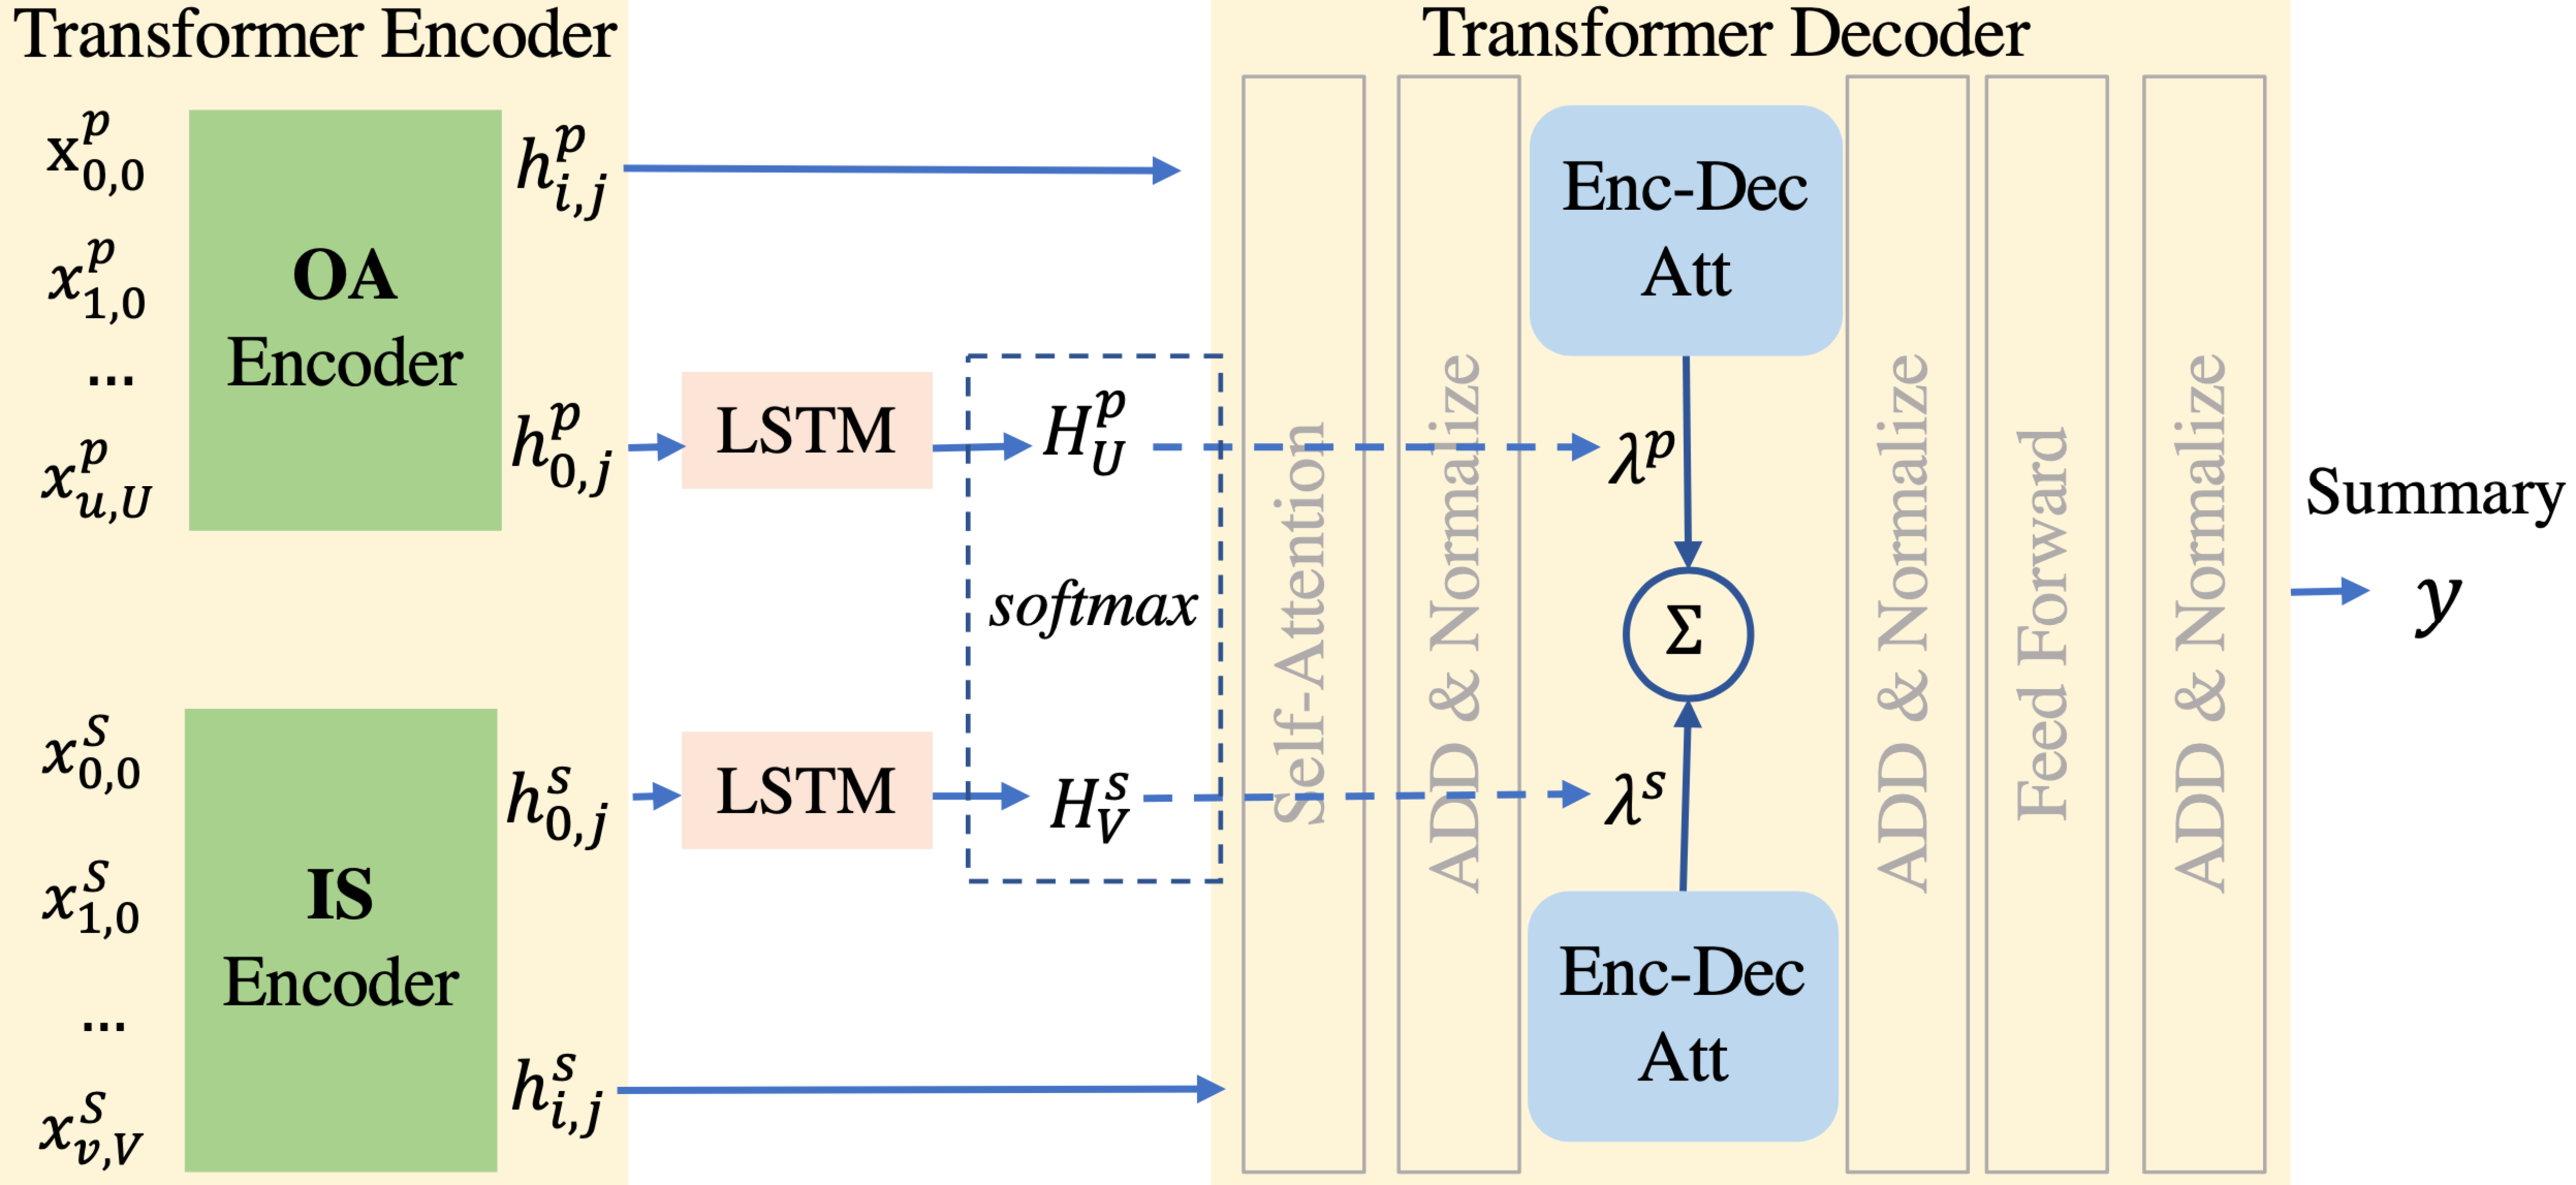
\includegraphics[width=1\linewidth]{./model.pdf}
	\caption{The architecture of MAI.}
	\label{fig:model}
\end{figure}
%We use the same methods to get
%noisy OAs embedding $\textbf{x}^p$=$(x^p_{0,0},x^p_{1,0},...,x^p_{u,U})$ 
%and noisy OSs embedding $\textbf{x}^s$=$(x^s_{0,0},x^s_{1,0},...,x^s_{v,V})$.
%We input noisy OAs to OA encoder and noisy ISs to IS encoder.
%$H^p_j$ and $H^s_{j'}$ is the encoder hidden state for $j$-th OA pair
%and $j'$-th IS sentence through LSTM layers.
%We take the last hidden state $H^p_U$ and $H^s_V$
%to represent opinion-aspect (generalized) information 
%and implicit sentences (specific) information.
We use $h^p_{i,j}$ and $h^s_{i',j'}$ to denote the encoder hidden state for $i$-th words in $j$-th OA pair
and $i'$-th word in $j'$-th IS sentence.
Inspired by~\citet{DialogMV2020},
we describe $j$-th OA pair in noisy OAs by 
the representation of $j$-th special token, $h^p_{0,j}$.
Then we aggregate the information of all pairs in noisy OAs through LSTM 
%~\cite{LSTM1997,DialogMV2020} 
as:
\begin{equation}
	\small
	H^p_j = LSTM(h^p_{0,j}, H^p_{j-1})
\end{equation}
%The last hidden state $H^p_U$.
where $H^p_j$ is the encoder hidden state for $j$-th OA.
We use the last hidden state $H^p_U$ as the OA representation.
Similary, we can get the IS representation $H^s_V$.
The {\em OA probability} $\lambda^p$ and 
{\em IS probability} $\lambda^s$ are calculated by:
\begin{equation}
	\small
	\tilde{H}^p_U = \tanh(WH^p_U+b) 
\end{equation}
\begin{equation}
		\small
	\tilde{H}^s_V = \tanh(W'H^s_V+b') 
\end{equation}
\begin{equation}
	\small
    \lambda^p = \frac{\exp(\tilde{H}^p_U {^\top} v^p)}{\exp(\tilde{H}^p_U {^\top} v^p)+\exp(\tilde{H}^s_V {^\top} v^s)} 
\end{equation}
\begin{equation}
\small
	\lambda^s = 1-\lambda^p 
\end{equation}
where $v^p$ and $v^s$ respectively denote the randomly initialized context vector of OA encoder and IS encoder.
$W$ and $b$ are parameters.
At each decoding step $t$, 
$C_t^p$ is the weighted sum of encoder hidden states of OA with Encoder-Decoder Attention (Enc-Dec Attn) as weight. 
$C_t^s$ is the weighted sum of IS encoder.
The combinational context vector $C_t$ for decoding is:
%of the Encoder-Decoder Attention 
%is the weighted sum of $C_t^p$ and $C_t^s$ as:
%is computed as:
%The combinational context vector $C_t$ for decoding is:
\begin{equation}
		\small
	C_t = \lambda^p C_t^p +  \lambda^s C_t^s
\end{equation}
%In this model, the decoder hidden state of MAGOS is $\mathbf{Z}=(Z_0,...,Z_T)$. The decoder state at timestep $t+1$ should be calculated from
%$Z_t$ and $C_t$. 
%We also use the $softmax$ function to compute the probability distribution of 
%generation over $\mathbf{Z}$.
%The probability distribution over vocabulary of decoder is the same as Equation \ref{eq:decode}.

\subsubsection{Training}
\label{sec:training}
For optimization, we first train BAG to learn the generalized information from noisy OAs.
Summaries generated by BAG
contain more accurate opinions and avoid 
losing important aspects.
Then, we further fine-tune MAI based on the pretrained
BAG. 
In this way, the generated summary is enhanced with
specific information from noisy ISs.


%We extract OAs and ISs of multi-review as noisy OAs and noisy ISs,
%which are the input of models.
%The human-written summaries are output.



